\chapter{Towards Parameter Learning}
\label{sec:parametric_learning_pra_model}

PRAs invariably involve uncertainty. When explicitly modeled, these uncertainties can be updated or inferred from evidence, engineering judgments, or reliability targets. We refer to such systematic updating of probability or frequency distributions across the PRA model as form of parametric learning.

Recall from (Section~\ref{sec:unified_pra_dag}) that we represent a PRA model as a PDAG. Let \(\boldsymbol{\theta}\) be the collection of parameters governing all relevant probabilities/frequencies in this PDAG. For an end-state \(S_j\), the model-based prediction under \(\boldsymbol{\theta}\) is
\[
P_{\mathcal{M}}\bigl(S_j \mid \boldsymbol{\theta}\bigr).
\]
If one also has observed or target frequencies \(\bigl\{p_{j}^{\mathrm{obs}}\bigr\}\), parametric learning seeks to reconcile this information with the model’s predictions by updating \(\boldsymbol{\theta}\). In a Bayesian setting, one may specify a prior distribution over \(\boldsymbol{\theta}\) and update this prior to a posterior distribution via the likelihood of observed end-state frequencies or other system-level evidence. Alternatively, one may adopt an optimization-based approach: define a loss or cost function that measures the discrepancy between \(\{p_{j}^{\mathrm{obs}}\}\) and \(\{P_{\mathcal{M}}(S_j \mid \boldsymbol{\theta})\}\), then minimize this loss with respect to \(\boldsymbol{\theta}\). Both perspectives aim to systematically adjust the PRA model’s probabilistic parameters so that end-state frequencies (or other risk metrics) remain consistent with available data or requirements. 

In the next section, we show how parametric learning over the PDAG can be setup as a constrained optimization problem.

\section{Parameter Learning as Constrained Optimization}
\label{sec:opt_formalization}

Each node \(X_i\) in the PDAG has an associated parameter \(\theta_i\), gathered into a vector  
\[
\boldsymbol{\theta}
\;=\;
(\theta_1,\;\theta_2,\;\dots,\;\theta_n).
\]
For a set of end-states \(\{S_j\}_{j=1}^m\), the model’s predicted probability under \(\boldsymbol{\theta}\) is  
\[
p_{j}^{\mathrm{pred}}\bigl(\boldsymbol{\theta}\bigr)
\;=\;
P_{\mathcal{M}}\bigl(S_j \mid \boldsymbol{\theta}\bigr).
\]
Suppose observed or target frequencies \(\bigl\{p_{j}^{\mathrm{obs}}\bigr\}\) are given. A discrepancy measure  
\[
d\!\bigl(p_{j}^{\mathrm{obs}},\,p_{j}^{\mathrm{pred}}(\boldsymbol{\theta})\bigr)
\]
compares the model’s predictions to these values. One can also add a regularization term \(\Psi(\boldsymbol{\theta})\) to encode additional constraints such as engineering limits or prior information. Let \(\Omega\) denote the feasible set for \(\boldsymbol{\theta}\), enforcing domain-specific requirements (e.g., probability normalization). Parameter learning then becomes the following constrained optimization problem:
\[
\min_{\boldsymbol{\theta} \,\in\, \Omega} 
\quad 
\sum_{j=1}^m
d\!\Bigl(
   p_{j}^{\mathrm{obs}},\,
   p_{j}^{\mathrm{pred}}(\boldsymbol{\theta})
\Bigr)
\;+\;
\Psi(\boldsymbol{\theta}).
\]
A solution \(\boldsymbol{\theta}^{*}\) in \(\Omega\) is sought that minimizes overall discrepancy while respecting any additional constraints. Gradient-based methods (when \(d\) is differentiable) or other solvers can be employed.

\section{Case Study: EBR-II Liquid Metal Fire Scenario}
\label{sec:case_study_ebr2}
We apply the proposed optimization method to an event tree from the Experimental Breeder Reactor-II (EBR-II) Level I PRA \citep{chang_experimental_2018}. The potential initiating event is a leak in the piping loop of the reactor's shutdown cooler, which uses sodium-potassium (NaK) coolant. Air intrusion near NaK can cause fire hazards. The event tree, shown in Figure \ref{fig:ebr2_sdfr_et} enumerates whether (i)~the liquid-metal fire is detected in time (\(\text{LMFD}\)), (ii)~a reactor scram is successfully initiated (\(\text{RFIR}\)), (iii)~the fire is classified as severe or limited (\(\text{LLRF}\)), (iv)~a plant-level fire suppression system fails or succeeds (\(\text{SSSD}\)), and (v)~critical secondary systems remain operational (\(\text{SYSO}\)). These conditional events interact to form multiple end-states, labeled \(\text{SDFR-0}\) through \(\text{SDFR-8}\). Some end-states represent minimal impact (e.g., immediate fire detection and promptly executed scram), whereas others lead to more severe conditions (e.g., no detection and system failures yielding potential core damage).

\begin{figure}[h]
  \centering
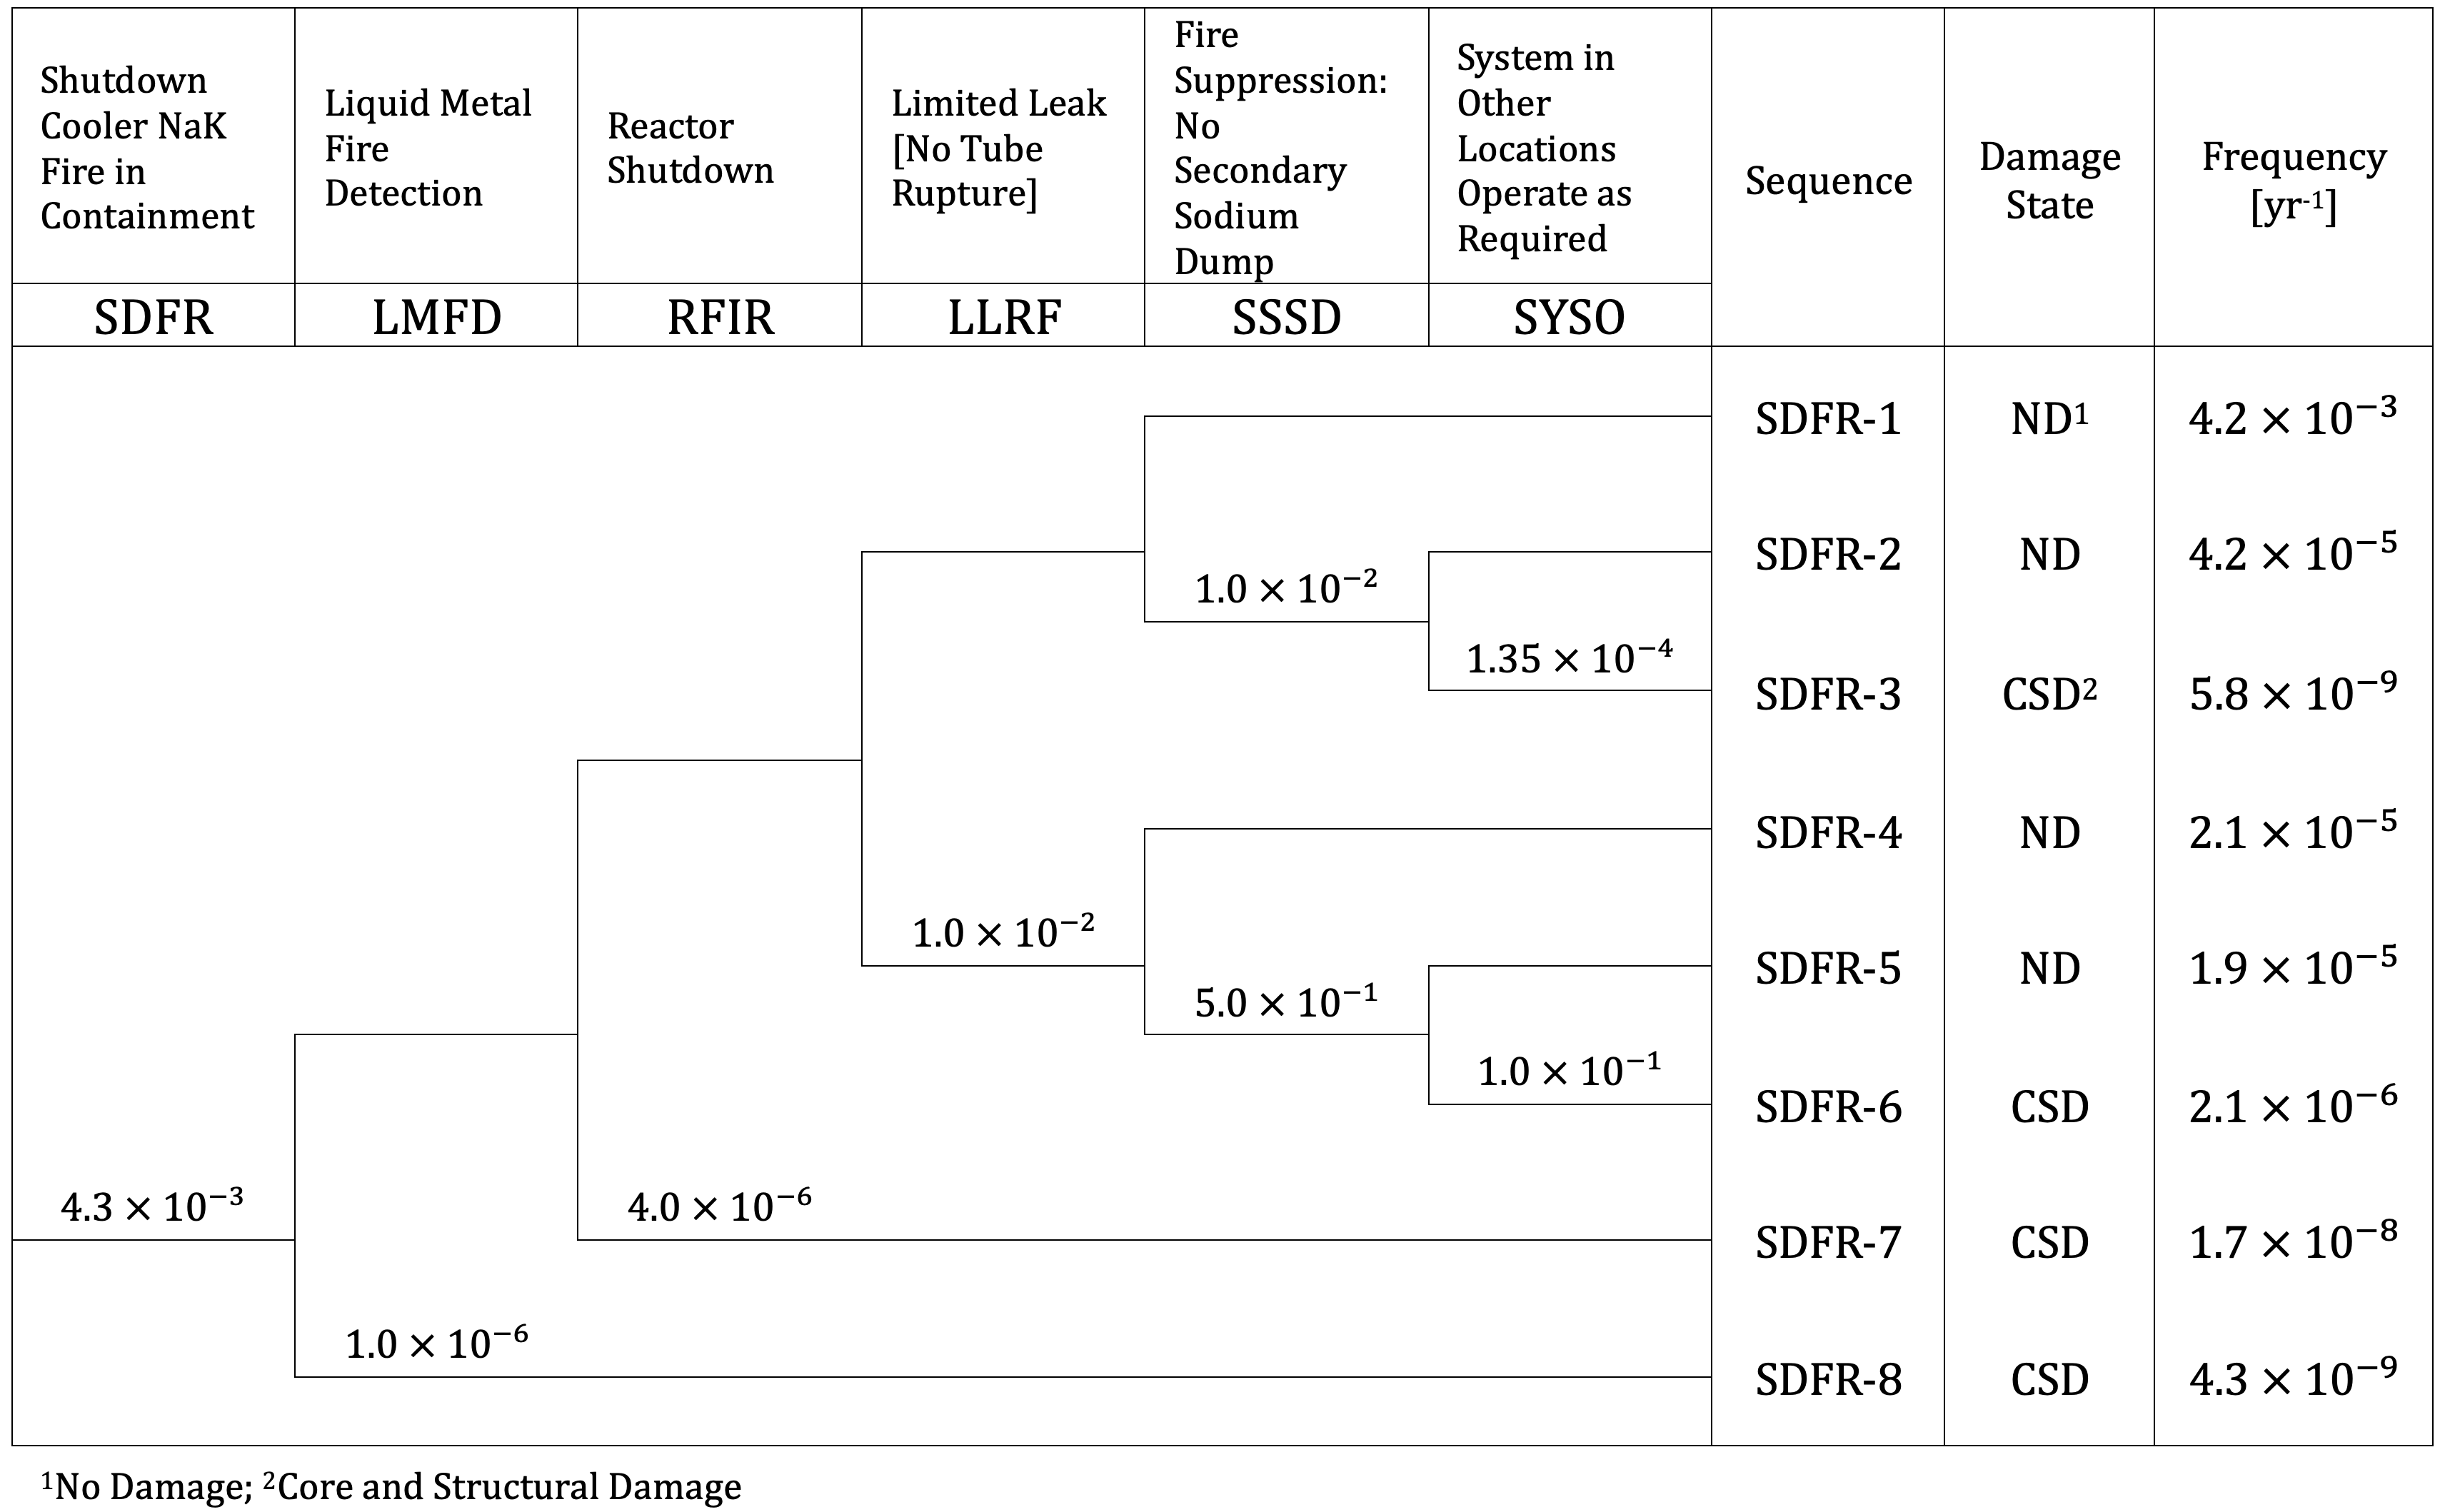
\includegraphics[width=1.0\textwidth]{parts/4_learning/1_param/figs/event_tree_NaK_fire.png} 
    \caption{EBR-II Shutdown Cooler NaK Fire in Containment}
    \label{fig:ebr2_sdfr_et}
\end{figure}

\subsection{Event Tree Structure and Problem Setup}
Following the notation from Section~\ref{sec:event_tree_definition}, each end-state \(S_j\) arises from a particular path of success/failure outcomes across the conditional events. Let \(\{X_1,\dots,X_n\}\) be the events (e.g., \(\text{LMFD}, \text{RFIR}, \dots\)), and let \(y_{ji}\in\{0,1,\text{NaN}\}\) indicate whether \(X_i\) fails, succeeds, or is not applicable for path \(S_j\). The probability of end-state \(S_j\) is
\begin{equation}
\label{eq:ebr2_es_probability}
P(S_j) 
\;=\;
\prod_{i=1}^{n} P\bigl(y_{ji}\bigr),
\end{equation}
where 
\begin{equation}
P\bigl(y_{ji}\bigr)
\;=\;
\begin{cases}
P\bigl[X_i = 1\bigr], & \text{if } y_{ji}=1,\\
1 - P\bigl[X_i = 1\bigr], & \text{if } y_{ji}=0,\\
1, & \text{if } y_{ji}=\text{NaN}.
\end{cases}
\label{eq:ebr2_conditional}
\end{equation}
Thus, one may represent each end-state \(S_j\) by multiplying the associated conditional event probabilities along its branch of the tree.

In this case study, each \(P\bigl[X_i=1\bigr]\) is assigned a (truncated) log-normal parameterization, reflecting the fact that event probabilities can span several orders of magnitude. Let \(\mu_i,\sigma_i\) denote the log-space mean and standard deviation of event \(X_i\). Under truncation rules (e.g., restricting \(\mu_i\in[10^{-10},1]\) and \(\sigma_i\in[10^{-10},10^{4}]\)), the resulting probability stays in \((0,1)\) and avoids extreme instabilities. These are plotted in Figure \ref{fig:conditionals_initial} as normalized kernel density estimates\cite{terrell_variable_1992}.

\subsection{Loss Function Definition}
Given a set of target or observed end-state frequencies \(\{p_{j}^{\mathrm{obs}}\}_{j=1}^m\), the task is to infer \(\{\mu_i,\sigma_i\}_{i=1}^n\) so that the predicted frequencies 
\[
p_{j}^{\mathrm{pred}}\;\equiv\;P\bigl(S_j \mid \{\mu_i,\sigma_i\}\bigr)
\]
match \(p_{j}^{\mathrm{obs}}\) as closely as possible. Denoting \(\boldsymbol{\theta}=(\mu_1,\sigma_1,\dots,\mu_n,\sigma_n)\) for all events, the optimal parameters solve a constrained minimization:
\begin{equation}
\label{eq:ebr2_optimization}
\min_{\boldsymbol{\theta}\in\Omega}
\quad
\mathcal{L}\bigl(\boldsymbol{\theta};\,\{p_{j}^{\mathrm{obs}}\}\bigr)
\quad
\text{subject to truncation and system constraints,}
\end{equation}
where \(\Omega\) encodes bounds (e.g., \(\mu_i,\sigma_i \ge 10^{-10}\)), and \(\mathcal{L}\) is a loss function. Here, one defines \(\mathcal{L}\) via a Normalized Relative Logarithmic Error (NRLE), which balances discrepancies in both the predicted end-state frequencies and the tails of the distributions. A simplified version of NRLE is:
\begin{equation}
\label{eq:ebr2_nrle}
\text{NRLE} 
\;=\;
\frac{1}{m}
\sum_{j=1}^{m}
\;\frac{1}{2}
\Bigl(
  \text{MAE}\bigl(\log[p_{j}^{\mathrm{obs}}+\epsilon],\,\log[p_{j}^{\mathrm{pred}}+\epsilon]\bigr)
  \;+\;
  \text{MAE}\bigl(\sigma_{j}^{\mathrm{obs}},\,\sigma_{j}^{\mathrm{pred}}\bigr)
\Bigr),
\end{equation}
where \(\text{MAE}\) denotes mean absolute error, and \(\epsilon\) is a small positive constant to avoid \(\log(\,0\,)\). The terms \(\sigma_{j}^{\mathrm{obs}}\) and \(\sigma_{j}^{\mathrm{pred}}\) refer to log-space standard deviations for the respective distributions of (or mapped from) end-states or functional events. By design, this objective penalizes deviations of both central tendencies and spread. A gradient-based algorithm (e.g., Adam \citep{zhang_improved_2018}) then iteratively refines \(\{\mu_i,\sigma_i\}\), using automatic differentiation with respect to \(\mathcal{L}\).

\subsection{Results \& Discussion}
\label{sec:results_and_discussion_estimation}
The parameter estimation recovered target distributions and corresponding end-state frequencies with near-accurate fidelity, indicating that the method is capable of approximating underlying probabilities from limited inputs. The predicted end-state frequency estimates are plotted in Figure \ref{fig:end-states_estimated}.

Specifically, end-state frequencies estimated under the constrained optimization process diverged from reported references by small margins: on average, the mean values were recovered with an error of about \((1.08\pm 0.96)\%\), the 5th percentile with \((4.39\pm 7.09)\%\), and the 95th percentile with \((3.82\pm 5.91)\%\).  Such deviations suggest that the overall approach captures the central tendencies of event probabilities reasonably well, while still exhibiting moderate scatter in both lower and upper distribution tails.  Recurrence of larger discrepancies in selected events (e.g., certain fire detection or suppression paths) emphasizes the known difficulty of accurately modeling rare failure or success probabilities—particularly when the choice of distribution (e.g., log-normal) imposes strong structural assumptions on the shapes of these probability curves.

Despite these promising quantitative metrics, two issues warrant discussion. First, although end-state frequencies are reproduced within small mean errors, there is a real possibility of overfitting to the specified targets.  The optimization-driven procedure can finely tune parameters to minimize a chosen loss function; however, doing so may lead to calibrated event probabilities that reflect artifacts of the objective rather than a physically robust representation.  This risk is heightened when dealing with low-probability events (e.g., a rare liquid metal fire condition combined with other system failures)—situations that often exhibit limited empirical data.  

Second, the truncation and bounds on the log-normal parameterization, while necessary for numerical stability, can restrict the feasible solution space in unintended ways.  Large or extremely small event probabilities, particularly in tail regions, must fit within these truncated distributions.  If the true system behavior lies outside the assumed bounds, the resulting estimates may systematically under- or overestimate important tail events.  This possibility is underscored by the modest underestimation observed at the 95th percentile for certain functional events in the demonstration.
\begin{landscape}
\begin{figure}[ht!]
  \centering
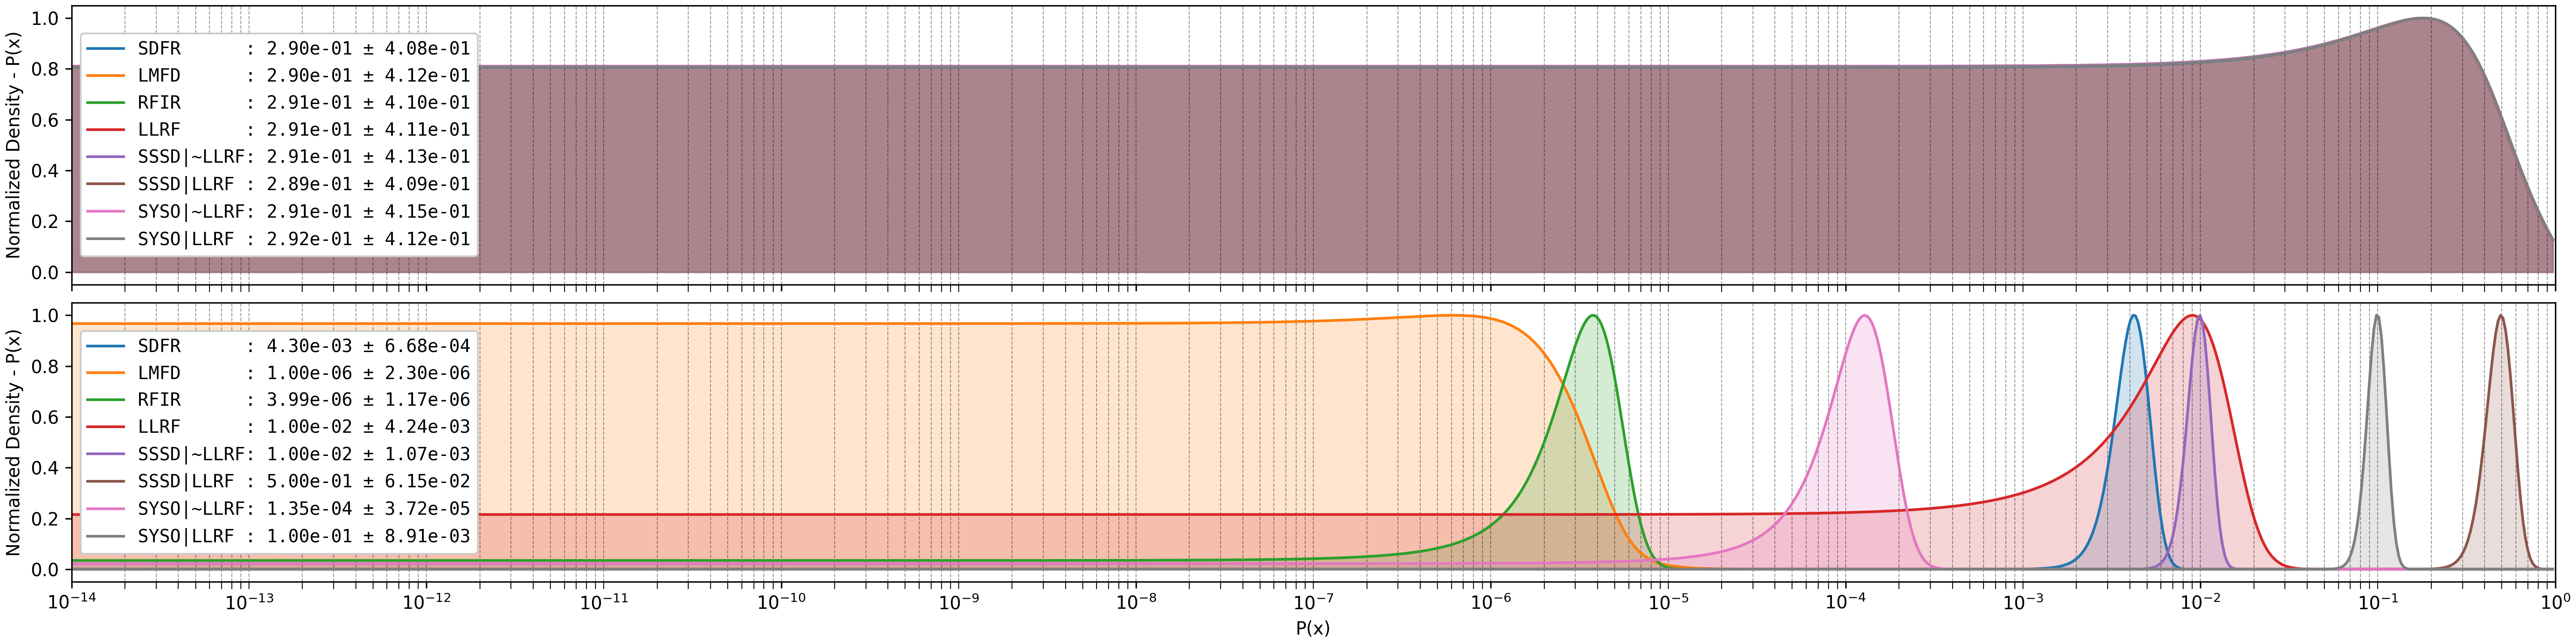
\includegraphics[width=\textwidth]{parts/4_learning/1_param/figs/conditional_events_prior.png}
    \caption{Initial vs Target Functional Event Probability Distributions}
    \label{fig:conditionals_initial}
\end{figure}

\begin{figure}[hb!]
\centering
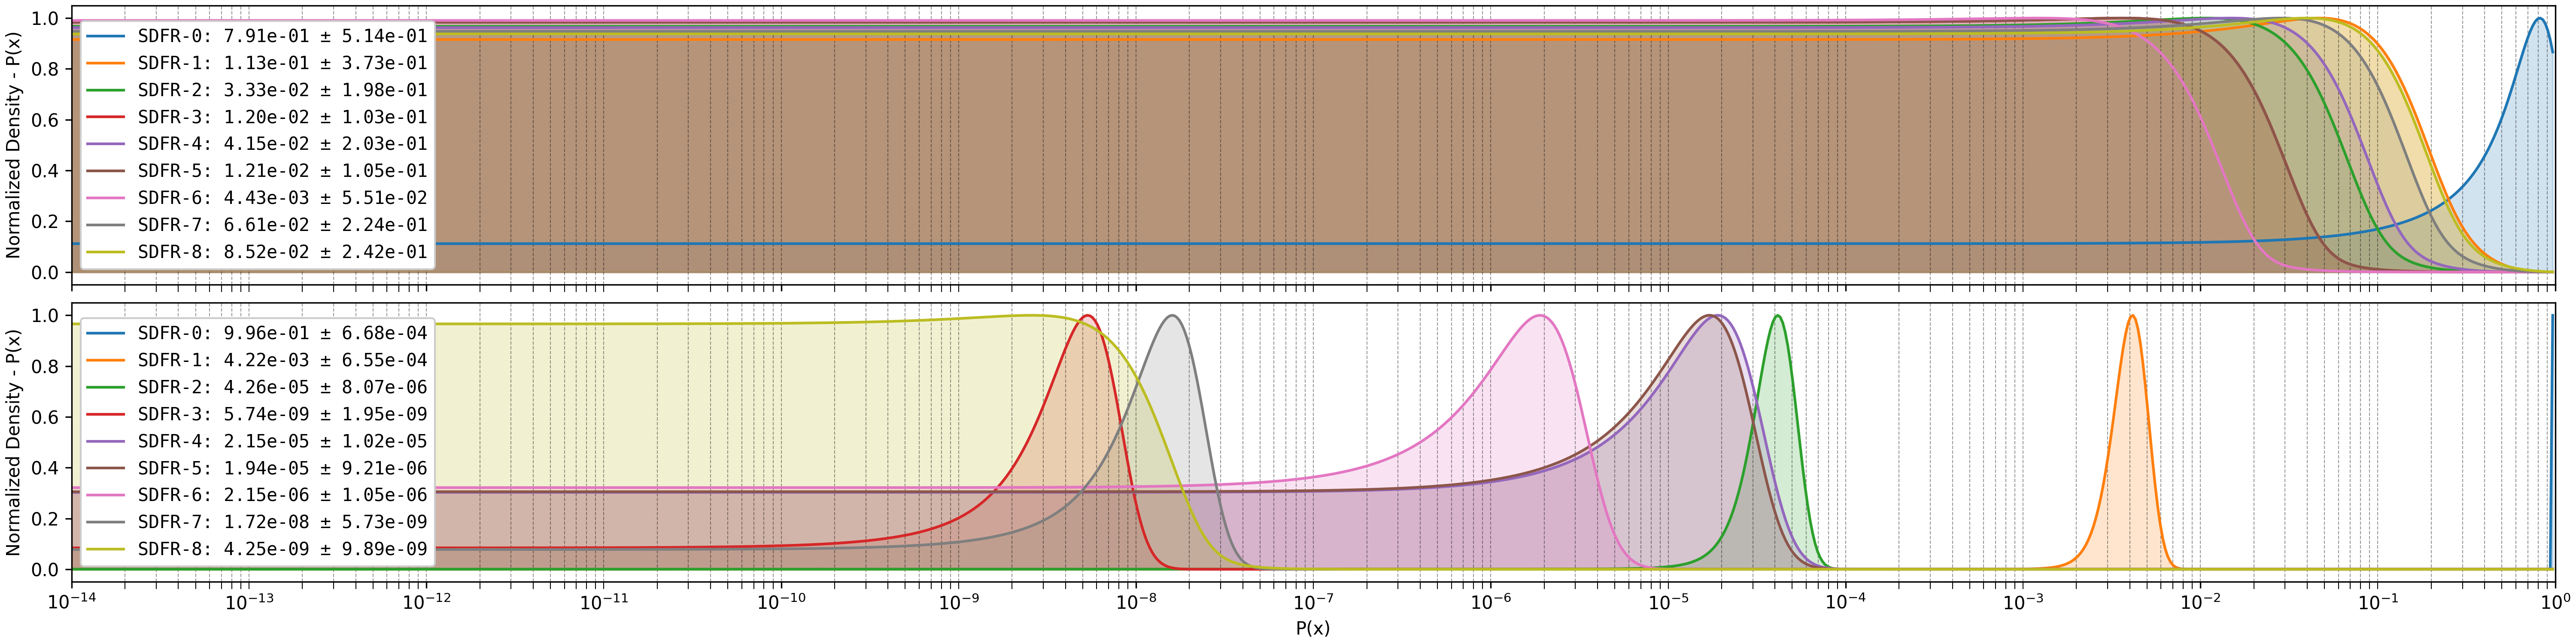
\includegraphics[width=\textwidth]{parts/4_learning/1_param/figs/end_states_prior.png}
    \caption{Initial vs Target End-State Frequency Distributions}
     \label{fig:end-states_initial}
\end{figure}
\end{landscape}

\clearpage
\begin{landscape}
\begin{table}[ht!]
\centering
\caption{Estimated vs Target Functional Event Probabilities Summarized}
\label{tab:conditional_estimated}
\scriptsize
\sisetup{table-format=1.2e-2}
\begin{tabular}{
    l
    S[table-format=1.2e-2]
    S[table-format=1.2e-2]
    S[table-format=1.2e-2]
    S[table-format=1.2e-2]
    S[table-format=1.2e-2]
    S[table-format=1.2e-2]
    S[table-format=1.2e-2]
    S[table-format=1.2e-2]
    S[table-format=1.2e-2]
    }
\toprule
\multirow{2}{*}{Event} & \multicolumn{3}{c}{$5^{th}$ Percentile} & \multicolumn{3}{c}{Mean} & \multicolumn{3}{c}{$95^{th}$ Percentile} \\
\cmidrule(lr){2-4} \cmidrule(lr){5-7} \cmidrule(lr){8-10}
& {Estimated} & {Target} & {Error\footnotemark} & {Estimated} & {Target} & {Error\footnotemark[\value{footnote}]} & {Estimated} & {Target} & {Error\footnotemark[\value{footnote}]} \\
\midrule
SDFR & 3.28e-03 & 3.30e-03 & -2.30e-05 & 4.24e-03 & 4.30e-03 & -5.97e-05 & 5.37e-03 & 5.47e-03 & -1.07e-04 \\
LMFD & 4.39e-08 & 4.29e-08 & 9.85e-10  & 1.00e-06 & 9.99e-07 & 7.13e-10  & 3.70e-06 & 3.70e-06 & -5.09e-09 \\
RFIR & 2.49e-06 & 2.39e-06 & 9.28e-08  & 4.13e-06 & 4.00e-06 & 1.29e-07  & 6.32e-06 & 6.15e-06 & 1.71e-07  \\
LLRF & 4.73e-03 & 4.72e-03 & 1.94e-05  & 9.93e-03 & 9.99e-03 & -6.36e-05 & 1.77e-02 & 1.79e-02 & -2.25e-04 \\
$\text{SSSD} \mid \overline{\text{LLRF}} $\footnotemark[2] & 8.72e-03 & 8.35e-03 & 3.68e-04  & 1.01e-02 & 1.00e-02 & 5.37e-05  & 1.15e-02 & 1.19e-02 & -3.31e-04 \\
$\text{SSSD} \mid \text{LLRF} $ & 4.93e-01 & 4.06e-01 & 8.74e-02  & 4.94e-01 & 5.00e-01 & -5.48e-03 & 4.96e-01 & 6.07e-01 & -1.11e-01 \\
$\text{SYSO} \mid \overline{\text{LLRF}} $ & 8.24e-05 & 8.33e-05 & -9.54e-07 & 1.36e-04 & 1.35e-04 & 8.31e-07  & 2.07e-04 & 2.03e-04 & 3.85e-06  \\
$\text{SYSO} \mid \text{LLRF} $ & 8.54e-02 & 8.60e-02 & -6.49e-04 & 9.89e-02 & 1.00e-01 & -1.11e-03 & 1.14e-01 & 1.15e-01 & -1.66e-03 \\
\bottomrule
\end{tabular}
\end{table}

\begin{figure}[hb!]
  \centering
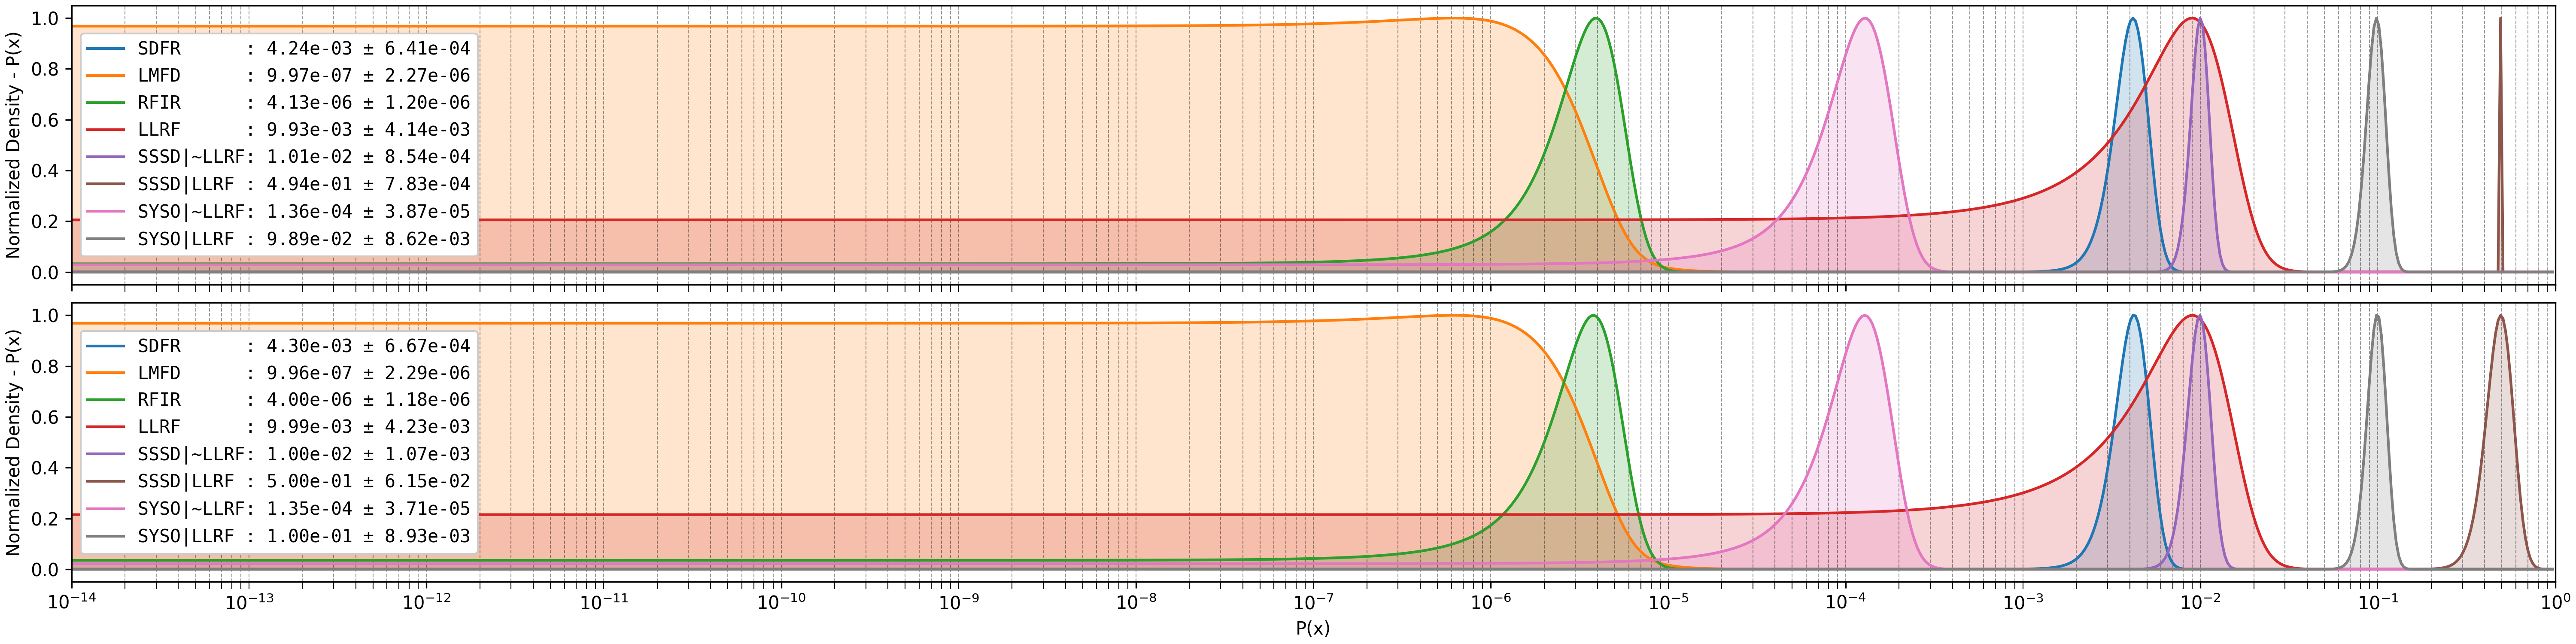
\includegraphics[width=\textwidth]{parts/4_learning/1_param/figs/conditional_events_predicted.png}
    \caption{Estimated vs Target Functional Event Probability Distributions}
    \label{fig:conditional_estimated}
\end{figure}

\footnotetext[1]{[Estimated - Target], negative values represent underestimates.}
\footnotetext[2]{$ A \mid \overline{B} $: event A conditional on the non-occurrence of event B.}
\end{landscape}
\clearpage

\clearpage
\begin{landscape}

\begin{table}[ht!]
\centering
\caption{Estimated vs Target End-State Frequencies Summarized}
\label{tab:summary}
\scriptsize
\sisetup{table-format=1.2e-2}
\begin{tabular}{
    l
    S[table-format=1.2e-2]
    S[table-format=1.2e-2]
    S[table-format=1.2e-2]
    S[table-format=1.2e-2]
    S[table-format=1.2e-2]
    S[table-format=1.2e-2]
    S[table-format=1.2e-2]
    S[table-format=1.2e-2]
    S[table-format=1.2e-2]
    }
\toprule
\multirow{2}{*}{Event} & \multicolumn{3}{c}{$5^{th}$ Percentile} & \multicolumn{3}{c}{Mean} & \multicolumn{3}{c}{$95^{th}$ Percentile} \\
\cmidrule(lr){2-4} \cmidrule(lr){5-7} \cmidrule(lr){8-10}
& {Estimated} & {Target} & {Error\footnotemark[3]} & {Estimated} & {Target} & {Error\footnotemark[\value{footnote}]} & {Estimated} & {Target} & {Error\footnotemark[\value{footnote}]} \\
\midrule
SDFR-0\footnotemark[4] & 9.95e-01 & 9.95e-01 & 1.08e-04 & 9.96e-01 & 9.96e-01 & 5.98e-05 & 9.97e-01 & 9.97e-01 & 2.30e-05 \\
SDFR-1 & 3.21e-03 & 3.23e-03 & -2.26e-05 & 4.16e-03 & 4.22e-03 & -5.86e-05 & 5.27e-03 & 5.37e-03 & -1.06e-04 \\
SDFR-2 & 3.12e-05 & 3.07e-05 & 5.81e-07 & 4.22e-05 & 4.26e-05 & -3.56e-07 & 5.52e-05 & 5.69e-05 & -1.70e-06 \\
SDFR-3 & 3.15e-09 & 3.15e-09 & -7.36e-12 & 5.73e-09 & 5.74e-09 & -1.31e-11 & 9.33e-09 & 9.35e-09 & -2.39e-11 \\
SDFR-4 & 9.62e-06 & 9.22e-06 & 4.07e-07 & 2.13e-05 & 2.15e-05 & -1.90e-07 & 3.94e-05 & 4.07e-05 & -1.33e-06 \\
SDFR-5 & 8.47e-06 & 8.31e-06 & 1.66e-07 & 1.88e-05 & 1.94e-05 & -5.87e-07 & 3.47e-05 & 3.67e-05 & -2.04e-06 \\
SDFR-6 & 9.10e-07 & 9.07e-07 & 3.35e-09 & 2.06e-06 & 2.15e-06 & -9.10e-08 & 3.85e-06 & 4.13e-06 & -2.86e-07 \\
SDFR-7 & 9.84e-09 & 9.58e-09 & 2.64e-10 & 1.75e-08 & 1.72e-08 & 3.08e-10 & 2.82e-08 & 2.79e-08 & 3.17e-10 \\
SDFR-8 & 1.81e-10 & 1.80e-10 & 1.85e-12 & 4.18e-09 & 4.24e-09 & -5.50e-11 & 1.56e-08 & 1.58e-08 & -2.53e-10 \\
\bottomrule
\end{tabular}
\end{table}

\begin{figure}[ht!]
\centering
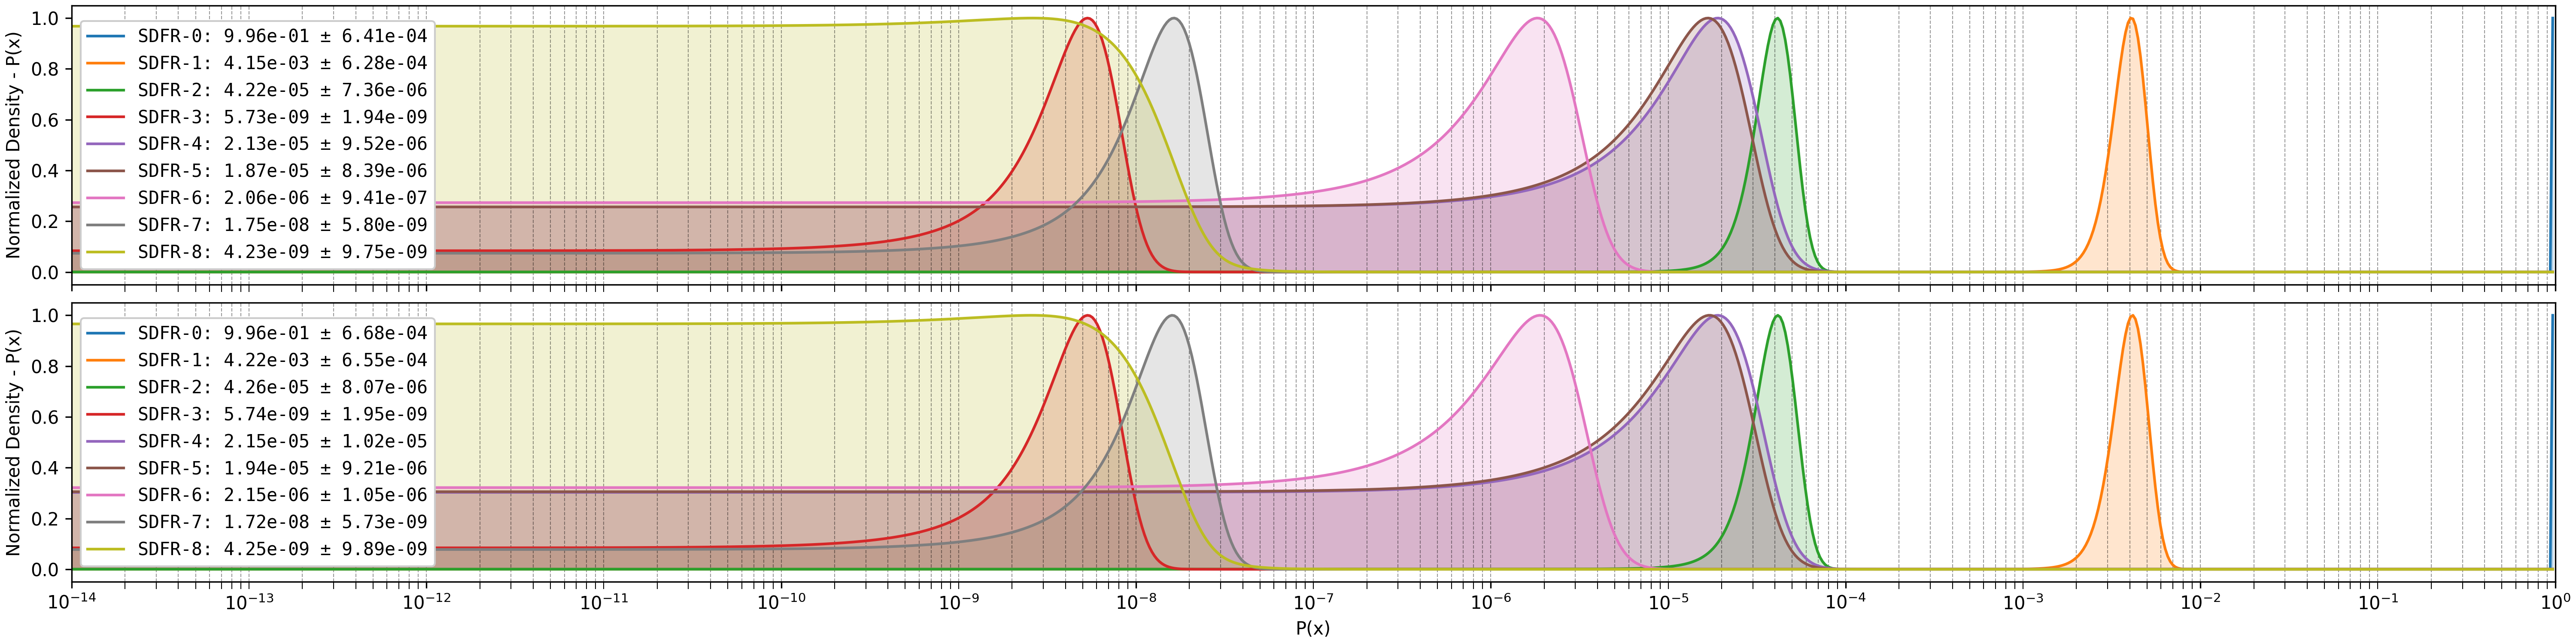
\includegraphics[width=\textwidth]{parts/4_learning/1_param/figs/end_states_predicted.png}
    \caption{Estimated vs Target End-State Frequency Distributions}
    \label{fig:end-states_estimated}
\end{figure}

\footnotetext[3]{[Estimated - Target], negative values represent underestimates.}
\footnotetext[4]{The likelihood of no SDFR. Computed by subtracting all end-state frequencies from the total probability.}
\end{landscape}
\clearpage
